\section{Experimental Results}
\label{section:experimental-results}

\begin{figure*}[ht]
  \subfigure[\emph{Pillar scenario} with an obstacle-evading prey\label{figure:learning_rate_pillar_dirchange}]{\includegraphics[width=0.24\textwidth]{plot_quality_learning-pillardir.eps}}\hfill\subfigure[\emph{Pillar scenario} with a predator-evading prey\label{figure:learning_rate_pillar_intelligent}]{\includegraphics[width=0.24\textwidth]{plot_quality_learning-pillarint.eps}}\hfill\subfigure[\emph{Random scenario} with a predator-evading prey\label{figure:learning_rate_random_intelligent}]{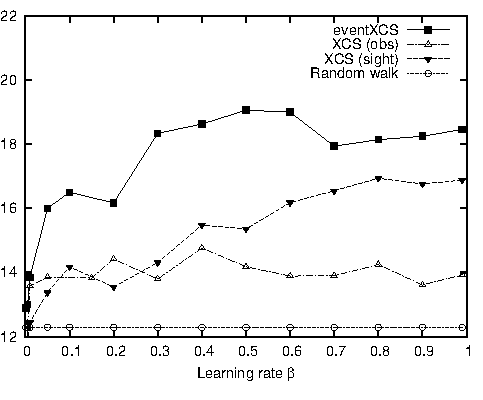
\includegraphics[width=0.24\textwidth]{plot_quality_learning-randint.eps}}\hfill\subfigure[\emph{Difficult scenario} with a blind prey\label{figure:learning_rate_difficult}]{\includegraphics[width=0.24\textwidth]{plot_quality_learning-difficult.eps}}\caption{\mathversion{bold}Comparison of different values for the learning rate $\beta$ for different XCS variants}\label{figure:learning_rate}
\end{figure*}

\begin{figure*}[ht]
  \subfigure[\emph{Pillar scenario} with an obstacle-evading prey\label{figure:experiment-pillardir}]{\includegraphics[width=0.24\textwidth]{plot_average_last_x_steps_goal_agent_observed-pillardir.eps}}\hfill\subfigure[\emph{Pillar scenario} with a predator-evading prey\label{figure:experiment-pillarint}]{\includegraphics[width=0.24\textwidth]{plot_average_last_x_steps_goal_agent_observed-pillarint.eps}}\hfill\subfigure[\emph{Random scenario} with a predator-evading prey\label{figure:experiment-randint}]{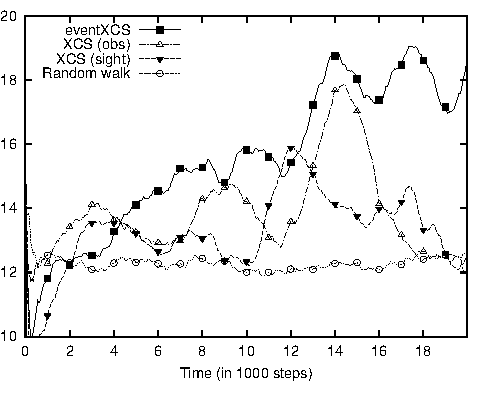
\includegraphics[width=0.24\textwidth]{plot_average_last_x_steps_goal_agent_observed-randint.eps}}\hfill\subfigure[\emph{Difficult scenario} with a blind prey\label{figure:experiment-difficult}]{\includegraphics[width=0.24\textwidth]{plot_average_last_x_steps_goal_agent_observed-difficult.eps}}\caption{\mathversion{bold}Comparison of the average quality over time of different XCS variants}\label{figure:experiments}
\end{figure*}

Many different design combinations of a reward function seems possible, as discussed before. This paper does not try to identify the best solution. Instead, it shows that there exists better implementations than the conventional XCS algorithm. Therefore, this paper concentrates on a comparison of XCS variants, as presented in Section~\ref{subsection:xcs-variants}. To properly compare this variants, it has been important to determine good parameter settings for each variant. While most of the standard values given in~\cite{BW02} and known as \emph{commonly used parameter settings} provide good results, some special settings need closer examination (see Section~\ref{subsection:xcs-parameters}). Thereby, thousands of different combinations have been tested and the parameter discussion could not completely presented in here. Configurations that achieved a lower performance than a simple \emph{random walk} strategy are also omitted since it is always difficult to argue whether the performance increase was caused by improved learning or by acting more like the \emph{random walk} strategy. For example in the \emph{random scenario} with an obstacle-evading prey the tested XCS were not able to show a significant better result than the \emph{random walk} strategy, so this scenario was omitted. Finally, the results of a number of experiments are presented in Section~\ref{subsection:experimental_results}.

%A major focus has been set on the comparison to a scenario, where predators completely behave on the base of randomized movements. Thus, all obtained results below such this random scenario have been rejected, since it is always difficult to argue, if a parameter setting with better results (and below the result of a random algorithm) just makes the predator's movements more random or if it actually learns better. The results of the parameter discussion are presented in Section~\ref{subsection:xcs-parameters}. 

\subsection{XCS Variants}
\label{subsection:xcs-variants}

All XCS variants that are presented here have in common that the corresponding scenario is not restarted when a positive reward was attained (as it is in the standard implementation of XCS). In all other aspects the first variant, which will be referred to as ``{\bf XCS (obs)}'', is equal to the standard implementation, i.e., the global goal is equivalent to the local goal and \emph{selfish behavior (observation range)} will be used (see Section~\ref{subsection:environment-reward-function}). Including more sensor information by using \emph{selfish behavior (sight range)} results in a new XCS variant which will be referred to as ``{\bf XCS (sight)}''. Combining this variant with event handling (see Section~\ref{subsection:events}) and using a reward distribution based on these generated events (see Section~\ref{subsection:reward-distribution}) results in an XCS variant which will be referred to as ``{\bf eventXCS}''. . Replacing also the selection strategy \emph{best selection} (see Section~\ref{section:learning-classifier-systems}) with \emph{tournament selection} (with a factor $p = 0.84$, see~\cite{Butz2003}) results in an XCS variant which will be referred to as ``{\bf eventXCS (ts)}''. Finally, using \emph{cooperative behavior}, results in the XCS variant ``{\bf eventXCS (coop, ts)}''.

%To summarize:
%XCS (obs): continously running standard implementation of XCS\\
%XCS (sight): XCS (obs) with reward function returns '1' when it is in sight\\
%eventXCS: XCS (sight) with events (see ...)\\
%eventXCS (tournament): eventXCS with tournament selection instead of best selection\\
%eventXCS (coll, tournament): eventXCS (tournament) with collaborative reward function\\


%showed in some scenarios significant better performance than any of the other XCS variants. In addition it is able to perform well with any of the tested environmental reward functions while XCS only works with a reward function modeled after the global goal. This will be referred to as ``{\bf SXCS}'' (\emph{Supervising eXtended Classifier System}).

\subsection{XCS Parameters}
\label{subsection:xcs-parameters}

\begin{figure}[ht]
\subfigure[\emph{Random} and {\emph pillar scenario} with obstacle- and predator-evading prey\label{figure:max-stack-size1}]{\includegraphics[width=0.23\textwidth]{plot_quality_maxstacksize1.eps}}\hfill\subfigure[
\emph{Difficult scenario} with blind prey and different \emph{eventXCS} variants\label{figure:max-stack-size2}]{\includegraphics[width=0.23\textwidth]{plot_quality_maxstacksize2.eps}}\hfill\caption{\mathversion{bold}Comparison of variants of \emph{eventXCS} with different \emph{maxStackSize} values in different scenarios}\label{figure:max-stack-size}
\end{figure}

%TODO: Bemerken, dass f�r Vergleich XCS / SXCS im difficult scenario hohe maxStackSize Werte besser sind

The parameter \emph{maxStackSize} that was introduced in Section~\ref{subsection:events} determines when a stack overflow (and thus a \emph{neutral event}) occurs. Similar to XCS' \emph{prediction discount} parameter $\gamma$, the optimal value is a compromise between several conflicting factors: Using larger values results in an inclusion of older - maybe irrelevant - actions in the reward of positive or negative events. Using smaller values can reduce the delay between an event and the actual reward but it may also lead to a possible disregard of actions that were important in achieving the current event. For scenarios with fewer obstacles and more open space (\emph{random} and \emph{pillar scenario}) a value between $4$ and $8$ seems optimal (see Figure~\ref{figure:max-stack-size1}) while in more complex scenarios like the \emph{difficult scenario} significant larger values up to $256$ seems optimal (see Figure~\ref{figure:max-stack-size2}). Additional tests showed that the size of the scenario is also relevant which might point to a correlation between the optimal value and the average distance to the prey. As a compromise and for better comparison a value of \emph{maxStackSize} $ = 8$ will be used in all tests.

%value does not have a large impact in the \emph{pillar} or \emph{random scenario}, only at around \emph{maxStackSize}~\( = 8\) a difference can be seen. The \emph{difficult scenario} on the other hand favors a larger value (\emph{maxStackSize}~\( = 32\)). In conclusion more complex routes to the goal probably require a larger value for \emph{maxStackSize}.

%\subsection{Learning rate $\beta$}\label{subsection:learning_rate}

During the tests another important parameter was the learning rate $\beta$. In a similar type of scenario in~\cite{1102281} a value below the standard value was proposed (\(\beta = 0.02\)). The reason was that dynamic multi-agent systems can be described only by movement probabilities so the learning process has to be slow and careful. Tests showed an optimal value of $0.05$ for the \emph{pillar scenario} (see Figure~\ref{figure:learning_rate_pillar_dirchange} and Figure~\ref{figure:learning_rate_pillar_intelligent}) and an optimal range of $0.6$ to $0.8$ for the \emph{random} and \emph{difficult scenario} (see Figure~\ref{figure:learning_rate_random_intelligent} and Figure~\ref{figure:learning_rate_difficult}). To maintain comparability between the scenarios and to other implementations of XCS a value of \(0.05\) was used for $\beta$ in further tests. 


According to~\cite{BW02} the maximum number of classifiers $N$ should be chosen big enough so that \emph{covering} happens only in the beginning of a run. For the scenario in question tests have shown that a population size of around $512$ fulfils this criteria. The classifier sets were filled with random classifiers~\cite{Butz2006} but no significant difference was seen. Instead sometimes a slower convergence was observed, probably because the corresponding system had to unlearn irrelevant classifiers. The \emph{GA threshold} parameter $\theta_{\mathrm{GA}}$ was set to $25$, larger values seemed to reduce the quality of the algorithm. As \emph{eventXCS} itself does use the quadratic reward distribution, the parameter \emph{reward prediction discount} $\gamma$ is only needed to compare XCS with \emph{eventXCS}. Tests have been inconclusive so the standard value of \(\gamma = 0.71\) was used. Only \(\gamma = 1.0\) showed significant different results in some cases. It seems that while a reduction of the transfer of the reward is needed, the actual value is of little importance. Other parameters, like the subsumption threshold $\theta_{\mathrm{sub}}$, GA threshold $\theta_{\mathrm{GA}}$ and the mutation probability $\mu$ values in the standard range were used ($20.0$, $25.0$ and $0.05$ respectively).


\subsection{Experimental results}\label{subsection:experimental_results}

The first result that can be seen in the graphs in Figure~\ref{figure:learning_rate} and Figure~\ref{figure:experiments} is that \emph{XCS (sight)} is always inferior to \emph{XCS (obs)}. Further tests with XCS in connection with different \emph{environmental reward functions} lead to the conclusion that XCS should not be combined with a reward function different than the global goal. On the other hand \emph{eventXCS} seems to work well with strategies like \emph{selfish behavior (sight range)}, which can be seen by the higher average quality of \emph{eventXCS} compared to \emph{XCS (obs)} and increasing learning curve in the scenarios displayed in Figure~\ref{figure:experiment-pillardir}, Figure~\ref{figure:experiment-pillarint} and Figure~\ref{figure:experiment-randint}. In addition, \emph{eventXCS} seems to be significantly more stable, i.e., it shows no tendency of overlearning or unlearning, as shown in the \emph{random scenario} in Figure~\ref{figure:experiment-randint}: \emph{eventXCS} reaches increasingly higher levels while \emph{XCS (obs)} breaks down after 14,000 steps. All in all in these three configurations \emph{eventXCS} is clearly superior to \emph{XCS (obs)}.
Looking further to the \emph{difficult scenario}, it can be seen that \emph{eventXCS} clearly fails, no matter to which value for the \emph{learning rate} $\beta$ is used (see Figure~\ref{figure:learning_rate_difficult}). This problem can only be solved by using the advanced variant \emph{eventXCS (ts)} or \emph{eventXCS (coop, ts)}. It shows again to be very stable compared to \emph{XCS (obs)} (see Figure~\ref{figure:experiment-difficult}) with the latter again failing after about 14,000 steps. All in all it is not surprising that \emph{XCS (obs)} reaches better results than \emph{eventXCS} because the former was designed to solve maze-like scenarios while \emph{eventXCS} was designed to solve a more open scenario with a non-blind moving prey. Because \emph{eventXCS} shares the same base algorithm with \emph{XCS (obs)} and because it can solve the \emph{difficult scenario} with \emph{tournament collection} it points to a flaw in the design of the algorithm that is correctable.

%Alternative implementations of SXCS with \emph{tournament selection} on the other hand solve the problem but reach only a lower level as XCS with \emph{best selection} (see Figure~\ref{figure:experiment-difficult}). But as in the \emph{random scenario} with a predator-evading prey XCS seems to have problems with overlearning. Increasing the learning rate $\beta$ to $0.2$ increase the quality in short-term, but in long-term XCS still has problems while SXCS present a very stable learning curve. In connection with a collaborative base reward function SXCS is even able to outperform XCS in the long run.\\

%Figure~\ref{figure:experiment-heuristics} show a comparison between possible static strategies. Collaborative strategies have just a small advantage over simple greedy strategies.

% show the average percentage of time steps where the prey was in observation range (each averaged over the last 2000 steps). With an predator-evading prey SXCS clearly outperforms XCS, while in the case with the obstacle-evading prey both variants show a similar learning curve. In all cases increasing the base reward function for XCS from observation range to sight range resulted in worse results.\\
%The case with an obstacle-evading prey in the \emph{random scenario} is not displayed, none of the XCS variants are able to gain a significant advantage over a ``random walk'' strategy.

%In Section~\ref{section:experimental-results} it was shown that SXCS outperforms XCS in scenarios with few obstacles. This was mainly due to the fact that XCS is unable to handle base reward functions that differ from the global goal and because XCS seems to have problems reaching a stable level, possibly due to overlearning. 
%SXCS with \emph{best selection} showed serious problems in the \emph{difficult scenario} while it was able manage the problem with a more random \emph{tournament selection}. This points to a correctable flaw in the design of the algorithm (probably with the \emph{neutral events}). But other than XCS SXCS \emph{can} handle advanced base reward functions, e.g. with a collaborative element (evading other agents) which significantly helps for example in the \emph{difficult scenario} though this is probably due to the fact that it simply encourages agents to move away from other agents, explore the grid and move through the openings. But in the end SXCS was designed to follow and observe a moving prey, the \emph{difficult scenario} is more like a labyrinth where finding the prey in the first place is important.
